\documentclass[conference]{IEEEtran}
\IEEEoverridecommandlockouts
\usepackage{cite}
\usepackage{amsmath,amssymb,amsfonts}
\usepackage{algorithmic}
\usepackage{graphicx}
\usepackage{textcomp}
\usepackage{xcolor}
\usepackage{booktabs}
\usepackage{array}
\usepackage{multirow}
\usepackage{url}

\def\BibTeX{{\rm B\kern-.05em{\sc i\kern-.025em b}\kern-.08em
    T\kern-.1667em\lower.7ex\hbox{E}\kern-.125emX}}

% Relax float placement parameters to keep figures in their respective sections
\renewcommand{\topfraction}{0.95}
\renewcommand{\bottomfraction}{0.95}
\renewcommand{\textfraction}{0.05}
\renewcommand{\floatpagefraction}{0.70}
\renewcommand{\dbltopfraction}{0.95}
\renewcommand{\dblfloatpagefraction}{0.70}

\begin{document}

\title{Domain-Specific Multi-Agent Retrieval-Augmented Generation with Closed-Loop Guardrail Verification for 5G New Radio and Open RAN Diagnostics}

\author{
\IEEEauthorblockN{Joyster Pinto (24BCE1245)}
\IEEEauthorblockA{\textit{School of Computer Science} \\
\textit{\& Engineering} \\
\textit{Vellore Institute of Technology}\\
Chennai, India \\
joyster.pinto2024@vitstudent.ac.in}
\and
\IEEEauthorblockN{Jeevith H C (24BCE5382)}
\IEEEauthorblockA{\textit{School of Computer Science} \\
\textit{\& Engineering} \\
\textit{Vellore Institute of Technology}\\
Chennai, India \\
jeevith.hc2024@vitstudent.ac.in}
\and
\IEEEauthorblockN{Dr. Vijayaprabakaran K}
\IEEEauthorblockA{\textit{School of Computer Science} \\
\textit{\& Engineering} \\
\textit{Vellore Institute of Technology}\\
Chennai, India \\
vijayaprabakaran.k@vit.ac.in}
}

\maketitle

\begin{abstract}
Fifth Generation New Radio (5G NR) and Open Radio Access Network (O-RAN) architectures introduce severe operational complexity. Network Operations Center (NOC) engineers expend up to 70\% of incident triage duration manually cross-referencing multi-layer telemetry alarms with dense 3GPP standards. While Large Language Models (LLMs) offer promising automated diagnosis, conventional Retrieval-Augmented Generation (RAG) fails due to domain acronym ambiguity, ungrounded telemetry parsing, and hallucinations of illegal configuration parameters. This paper presents an offline, multi-agent diagnostic framework for 5G NR and O-RAN infrastructures. The system incorporates a Dynamic Evidence-Weighted Reciprocal Rank Fusion (EWRRF) formulation coupling lexical BM25, dense semantic embeddings, cross-encoder re-ranking, and exact normative entity matching. A supervisor agent orchestrates dynamic task delegation across six protocol-specialized domain agents structured via a Directed Acyclic Graph (DAG). Furthermore, a closed-loop Stage 4 Guardrail Verifier enforces 3GPP TS 38.331 normative bounds and TS 28.541 neighbor congestion thresholds with automated reflection. Tested on consumer workstation edge hardware, the proposed framework achieves 87.5\% TeleQnA benchmark accuracy (+5.4\% over Telco-RAG), 100.0\% top-5 clause recall, and zero safety parameter violations.
\end{abstract}

\begin{IEEEkeywords}
5G New Radio, O-RAN, 3GPP Technical Specifications, Retrieval-Augmented Generation, Multi-Agent Systems, Directed Acyclic Graph, Root Cause Analysis, Self-Organizing Networks, Guardrail Verification, Quantized LLMs.
\end{IEEEkeywords}

\section{Introduction}

\subsection{Domain Background}
Fifth Generation New Radio (5G NR) and Open Radio Access Networks (O-RAN) represent highly intricate distributed infrastructures. With global 5G connections exceeding 1.6 billion, base station densification has grown by over 300\% to support URLLC and mMTC services. Consequently, monolithic base stations have transitioned toward disaggregated topologies where radio functions are decoupled into Centralized Units (O-CU), Distributed Units (O-DU), and Radio Units (O-RU) coordinated by Near-Real-Time and Non-Real-Time RAN Intelligent Controllers (RIC) \cite{polese2023}.

While disaggregation enhances multivendor flexibility, operational complexity escalates dramatically. Over 3,000 active 3GPP and O-RAN specifications spanning Releases 15--18 define more than 250,000 pages of interrelated protocol states, timers, and procedures \cite{ts38331, ts38213, oran_e2ap}. Furthermore, physical radio degradations (e.g., uplink PUSCH interference or sudden SINR drops) trigger cascading alarm storms across the MAC, RRC, and transport layers. Studies indicate that NOC engineers spend up to 70\% of triage cycles manually correlating raw telemetry with specifications, creating severe operational bottlenecks.

\subsection{Limitations of Traditional Generative Models}
Conventional foundation models and generalist RAG pipelines exhibit three fundamental deficiencies in cellular operations \cite{maatouk2024}: 1) Acronym and Entity Ambiguity: General models frequently conflate RRC protocol timers with O-RAN functional split parameters; 2) Unbounded Parameter Hallucinations: Unverified generative adjustments (e.g., increasing Cell Individual Offsets toward cells experiencing physical resource block exhaustion) trigger call drops and network-wide handover oscillations; 3) Data Sovereignty and Edge Constraints: Cloud-hosted APIs violate strict telecommunication privacy mandates and introduce unacceptable transit latency.

\subsection{Problem Statement}
The objective is to process heterogeneous multi-modal inputs, including operator inquiries, multi-cell KPIs (SINR, BLER, RSRP, PRB usage), and semi-structured alarms (handover expirations, RACH collisions, NGAP drops), to perform automated root cause analysis and synthesize actionable 3GPP-grounded remediation. The framework must operate completely offline on consumer edge hardware without cloud reliance, ensuring data sovereignty while mathematically guaranteeing parameter safety.

\subsection{Key Contributions}
This paper introduces four primary architectural contributions:
\begin{enumerate}
    \item A Dynamic Evidence-Weighted Reciprocal Rank Fusion (EWRRF) formulation integrating lexical BM25, dense embeddings, cross-encoder re-ranking, and exact 3GPP timer evidence matching.
    \item A Directed Acyclic Graph (DAG) task delegation engine decomposing multi-layer incidents across 6 protocol-specialized domain agents.
    \item A closed-loop Stage 4 Guardrail Verifier enforcing 3GPP TS 38.331 normative bounds and TS 28.541 neighbor congestion limits with reflective feedback.
    \item A fully offline edge deployment powered by a quantized Qwen 2.5 3B Instruct model executing on a consumer GPU workstation.
\end{enumerate}

\begin{table*}[t]
\centering
\caption{Comparative Summary of Top Reviewed Literature in Telecom RAG and Multi-Agent Diagnostics}
\label{tab:lit_survey}
\renewcommand{\arraystretch}{1.22}
\begin{tabular}{p{0.8cm} p{0.7cm} p{1.8cm} p{2.6cm} p{3.6cm} p{2.7cm} p{3.4cm}}
\toprule
\textit{Ref.} & \textit{Year} & \textit{Authors} & \textit{Dataset / Domain} & \textit{Core Methodology} & \textit{Key Metric} & \textit{Key Observation} \\
\midrule
\cite{bornea2024} & 2024 & Bornea \textit{et al.} & 3GPP Rel 15--18 \& TeleQnA & Hybrid BM25 and Dense RAG with Acronym Glossary & Top-5 Recall: 88.4\%, QA Acc: 82.1\% & Single-agent system; cannot parse live RAN alarms. \\
\cite{yilma2024} & 2024 & Yilma \textit{et al.} & 3GPP TS 38 Series & Section-preserving token chunking \& Vector Search & MRR: 76.2\%, P@5: 84.5\% & Struggled to answer questions across multiple specifications. \\
\cite{maatouk2024} & 2024 & Maatouk \textit{et al.} & TeleQnA (10,000 MCQs) & Benchmark evaluation of LLMs on Telecom Standards & Baseline LLM Acc: 61.2\%--78.4\% & General models struggle with timers and dense acronyms. \\
\cite{gajjar2025} & 2025 & Gajjar \textit{et al.} & 5G Core \& RAN Telemetry & Multi-Agent Tool-Chaining System (Tele-LLM-Hub) & Task Completion: 89.1\%, F1: 0.87 & Agents too generic; no specialists in RRC, PHY, or O-RAN. \\
\cite{liu2025} & 2025 & Liu \textit{et al.} & 5G NFV Alarms & Multi-Agent Log Parsing for Root Cause Analysis & RCA Top-1 Accuracy: 81.4\% & Focused on Core alarms; lacks SINR and handover rules. \\
\cite{zhou2024} & 2024 & Zhou \textit{et al.} & Multi-Cell 5G RAN Logs & In-Context SON Optimisation for Mobility and Tilt & HO Drop Reduction: 22.5\% & Cannot provide valid 3GPP clause references. \\
\cite{zhao2026} & 2026 & Zhao \textit{et al.} & O-RAN Near-RT RIC Logs & Multi-Agent System with Safety Boundaries & Safety Issues: 0\% & Numeric controller only; no natural language RAG or Q\&A. \\
\bottomrule
\end{tabular}
\end{table*}

\section{Literature Survey}
This section provides an overview of recent advances in domain-specific language modelling, retrieval-augmented generation, multi-agent network diagnosis, and root cause analytics.

\subsection{Survey of Existing Research}
1) Bornea \textit{et al.} (2024) \cite{bornea2024} developed a specialized retrieval system for answering questions about 3GPP Releases 15--18 specifications using the Telco-RAG framework. This used a telecom acronym dictionary, with a combination of lexical and dense retrieval strategies to increase the relevance of answers. They achieved high results for static multiple-choice questions, but the system was a single-agent architecture unable to read live telemetry data.

2) Yilma \textit{et al.} (2024) \cite{yilma2024} developed a system called TelecomRAG which uses a hierarchical chunk and dense vector search system to identify information from the 3GPP TS 38 series. They tuned their chunking strategy to retain section titles, increasing both their mean reciprocal rank and clause search accuracy. However, this did not take into account the state machine of protocols and failed to answer questions when multiple specifications needed to be searched.

3) Maatouk \textit{et al.} (2024) \cite{maatouk2024} created the TeleQnA dataset containing 10,000 questions about telecommunications. They discovered that general foundation models fail at answering questions related to numerical values such as frequency bands, timers, and signalling processes. This provided baseline results for general and domain-specific models.

4) Gajjar \textit{et al.} (2025) \cite{gajjar2025} developed a multi-agent system called Tele-LLM-Hub to automate telecommunications by using tools. This showed that by breaking down queries into multiple agents, the task completion rate is increased. However, the agents were too generic and did not have any agents specialised in different radio protocol areas such as physical layer quality.

5) Liu \textit{et al.} (2025) \cite{liu2025} developed a root cause analysis system called TN-AutoRCA to reduce alarm storms and identify the main problem nodes. This used a pipeline to break down log parsing and reasoning to reduce repair time. However, they could not provide much insight into radio access network issues such as uplink interference.

6) Zhou \textit{et al.} (2024) \cite{zhou2024} looked into automating network optimisation using SON-LLM. This used in-context retrieval to give advice on mobility and coverage settings. They saw improvements in edge throughput and fewer handover drops. However, this did not use any section-level references from 3GPP specifications and could not answer general questions.

7) Zhao \textit{et al.} (2026) \cite{zhao2026} looked at how to ensure safety in multi-agent systems using the O-RAN Near-Real-Time RAN Intelligent Controller. This used a deterministic boundary check to ensure zero safety issues. This is reliable when dealing with numerical values, but does not provide any natural language explanation and cannot retrieve explanations from standard documents.

8) NetLLM was proposed by Wu \textit{et al.} (2024) \cite{wu2024}. This framework enables foundation models to perform low-level networking functions through parameter-efficient fine-tuning and prompt engineering. Experiments were undertaken across adaptive bitrate streaming and cluster job scheduling, showing that smaller 8B parameter models can understand network state telemetry. However, this was focused around transport-layer scheduling, rather than diagnosing root causes of problems through natural language or evaluating 3GPP standards.

9) Du \textit{et al.} (2024) \cite{du2024} proposed a collaborative multi-agent solution for 6G intent-driven networks using game theory to coordinate tasks. Breaking down complex intents into sub-agents improved latency and accuracy of translating an intent. Whilst this has strong mathematical foundations, there was no direct integration with normative 3GPP documents, precluding evaluation of radio resource control signalling constraints.

10) A Graph-RAG solution was developed by Wang \textit{et al.} (2024) \cite{wang2024}, which used network graph representations to reduce hallucination. By representing relationships between base stations as triplets, false claims made during cellular diagnostics were reduced. However, the knowledge graph was static, preventing incorporation of dynamic 3GPP Release 17 and Release 18 clauses.

11) Polese \textit{et al.} (2023) \cite{polese2023} provided an extensive study of the Open RAN architecture, detailing functional splits across central, distributed, and radio units and examining control loop operations across E2, O1, and A1 interfaces. This offers a fundamental baseline for control-loop timing in Near-RT and Non-RT RIC controllers; however, an interactive standards-grounded search mechanism was not incorporated.

12) DeepSpecs was proposed by Xu \textit{et al.} (2024) \cite{xu2024}. This is a neuro-symbolic solution for verifying protocol implementations against specification documents. The solution achieved high levels of citation fidelity and logical consistency when analysing requests for comments and cellular specifications. However, it required large clusters of multi-GPUs to be used, meaning it could not be deployed offline.

13) Causal-LLM was investigated by Chen \textit{et al.} (2025) \cite{chen2025}. This solution uses causal graph discovery and language model explanations to identify anomalies. By identifying relationships between signal loss in the physical layer and uplink interference, explanations were made clearer to field engineers. However, this only provided explanations for faults and could not generate self-organising network parameter changes.

14) Sun \textit{et al.} (2025) \cite{sun2025} designed a topological-temporal graph transformer solution. This identified issues with fault propagation in dense 5G cells. The numerical classifier achieved a high F1-score for detecting anomalies with a low false alarm rate. However, this was a black-box solution lacking natural language reasoning and 3GPP clause references.

15) A calibrated 5G New Radio failure dataset was created by Al-Hourani \textit{et al.} (2025) \cite{alhourani2025}. This used two discrete-event simulators (Simu5G, OMNeT++) to simulate twelve different radio access failures, including handover timeout, random access preamble collision, and beam failure recovery. Whilst this provided realistic multi-cell telemetry data, it served solely as a simulation benchmark without diagnostic agent capabilities.

\subsection{Observations and Solution}
From the comparative literature analysis summarized in Table~\ref{tab:lit_survey}, two primary technological limitations become evident in current telecommunications AI frameworks:
\begin{enumerate}
    \item Disjointed Architecture: Existing solutions either operate solely as text-based document retrieval systems or function as isolated numerical anomaly detectors, lacking the architectural synthesis required to bridge raw telemetry alarms with normative standards clauses.
    \item Absence of Closed-Loop Parameter Verification: Prevailing generative models generate configuration recommendations without validating neighboring cell capacity constraints or normative 3GPP specification limits, introducing unacceptable operational risks into production cellular deployments.
\end{enumerate}

To overcome these fundamental limitations, this paper establishes a unified 5-stage domain-specific multi-agent architecture incorporating Dynamic Evidence-Weighted Reciprocal Rank Fusion (EWRRF) and a Closed-Loop Guardrail Verifier. The framework couples hybrid confidence-weighted document retrieval with reflective feedback between the verification engine and supervisor agent, simultaneously achieving high retrieval precision and mathematically verified self-healing remediation.

\begin{figure*}[p]
\centering
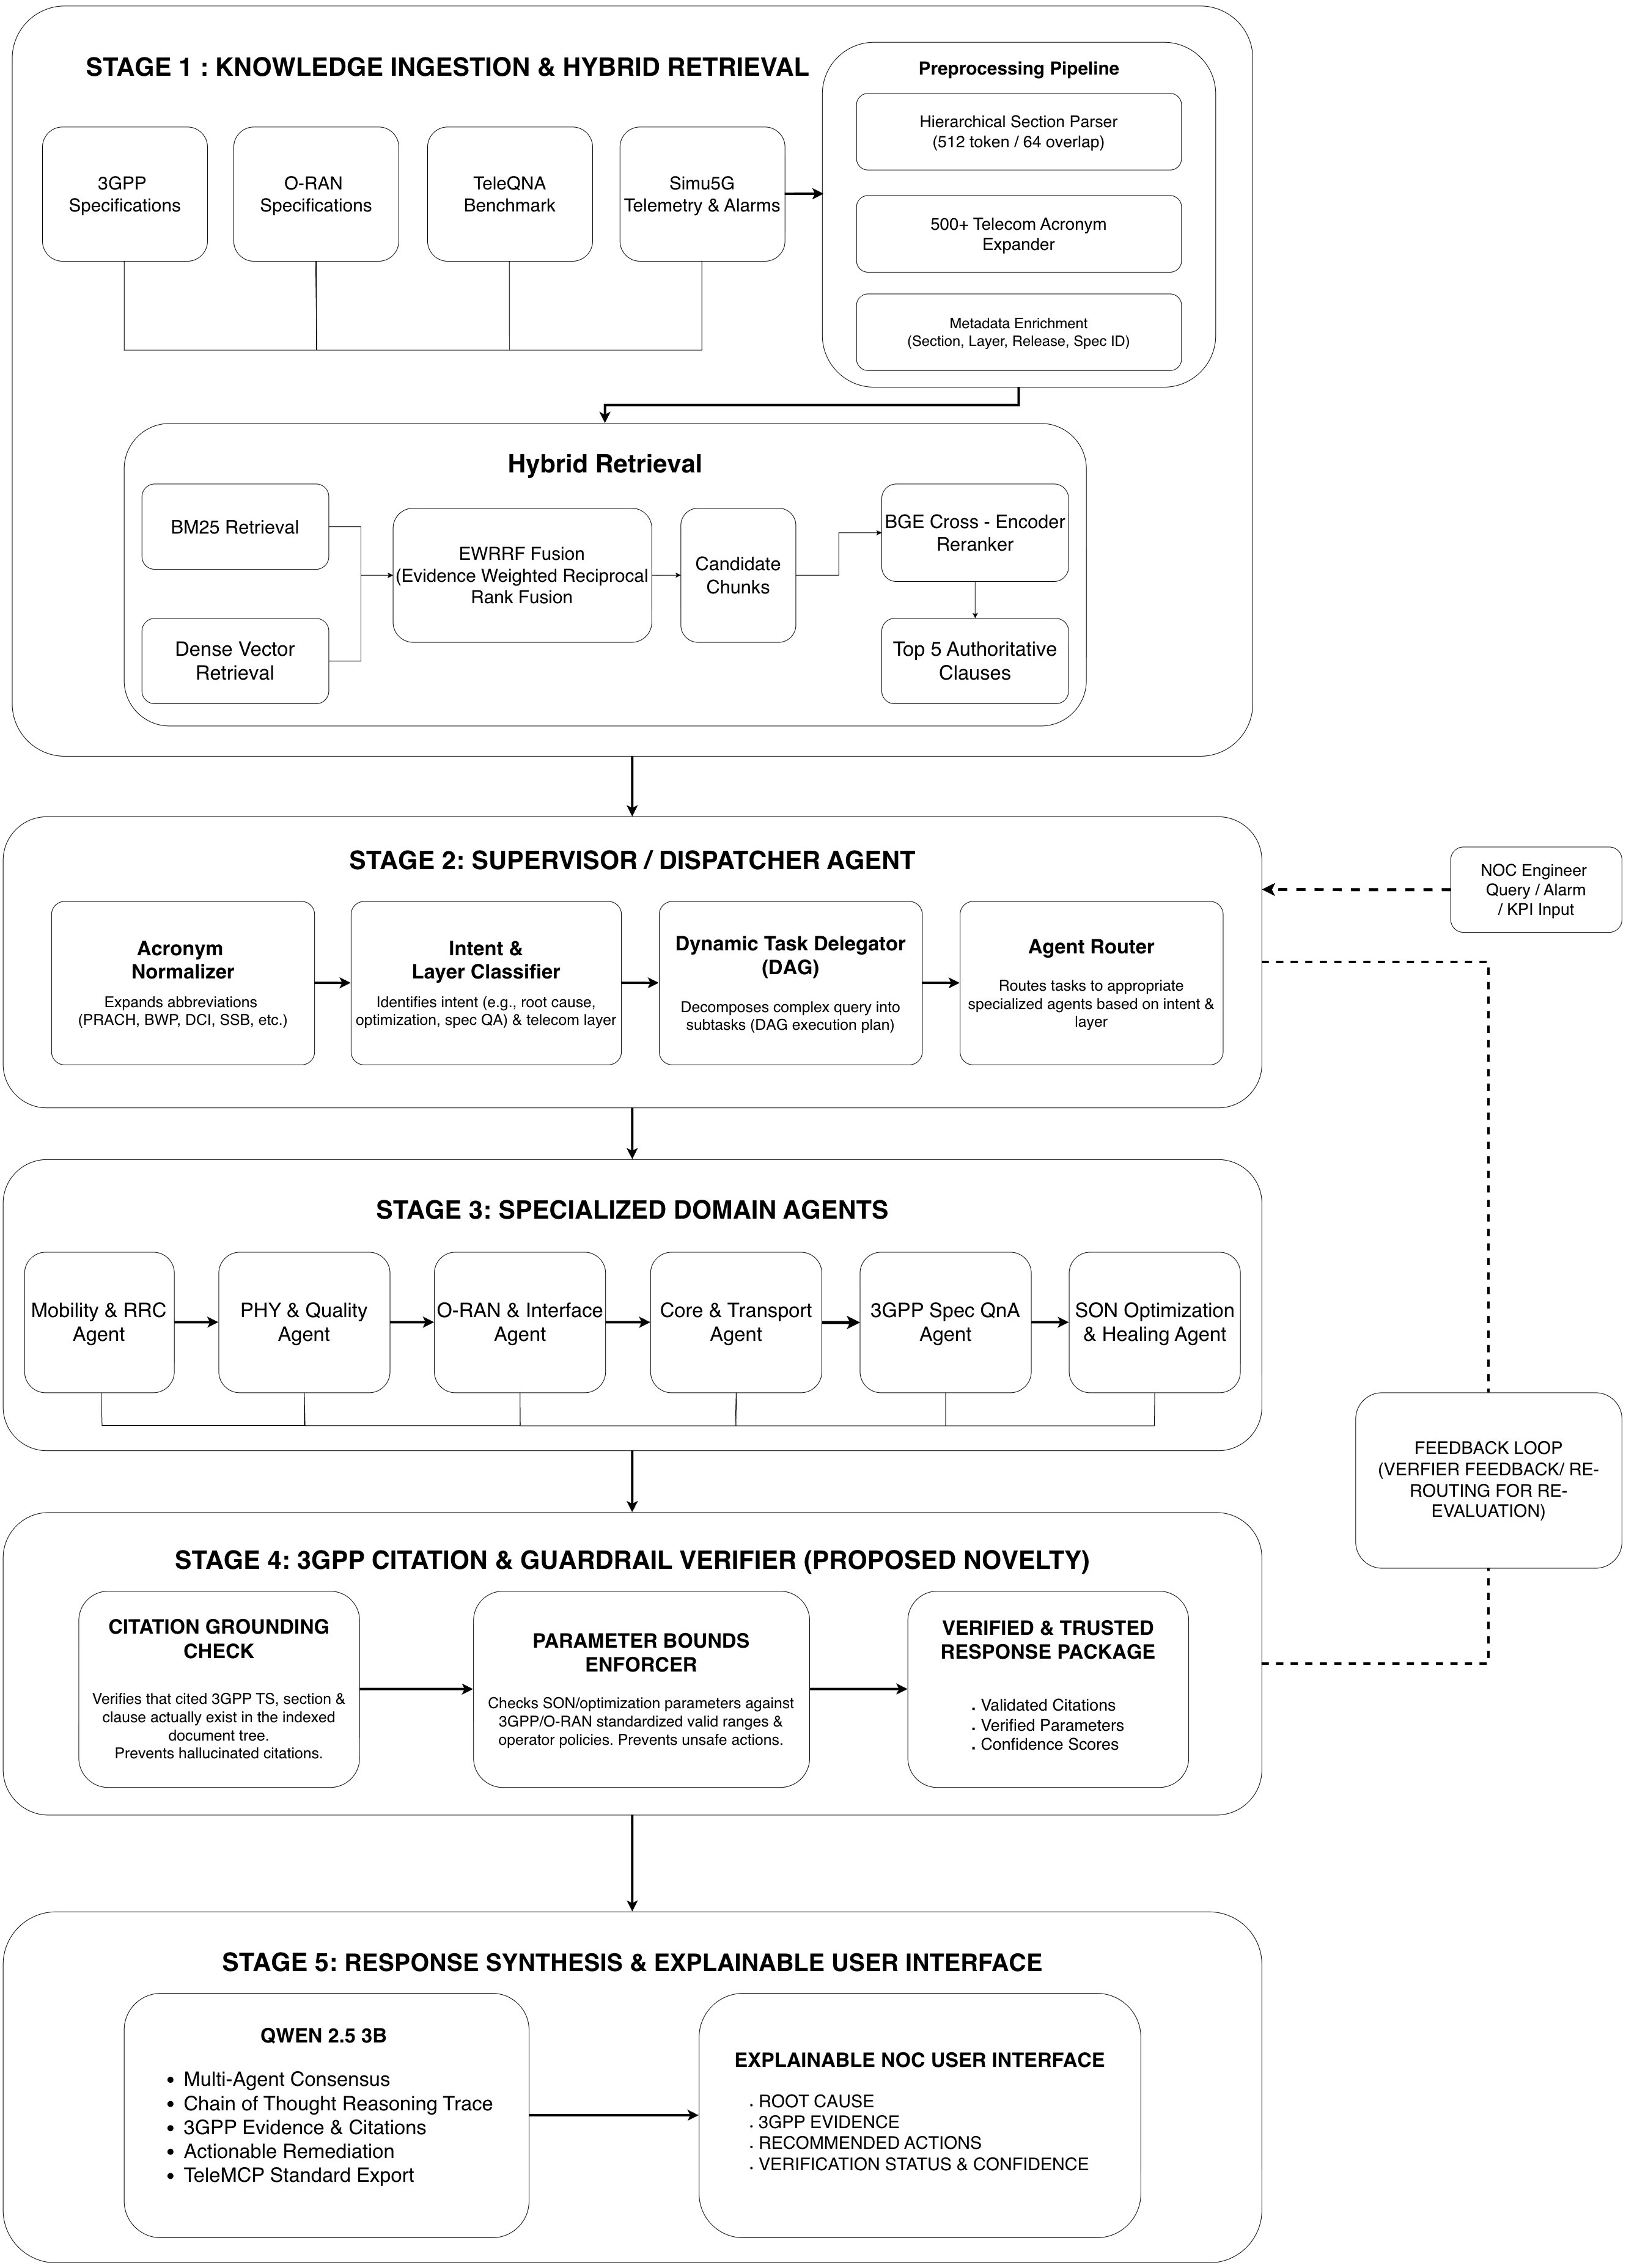
\includegraphics[width=0.92\textwidth, height=0.88\textheight, keepaspectratio]{figures/pipeline.jpeg}
\caption{Proposed 5-Stage Multi-Agent System Architecture featuring Dynamic Evidence-Weighted Reciprocal Rank Fusion (EWRRF), Directed Acyclic Graph (DAG) Task Delegation, 6 Protocol Specialist Agents, and the Stage 4 $\rightarrow$ Stage 2 Closed-Loop Guardrail Verification Path.}
\label{fig:architecture}
\end{figure*}

\section{Proposed Methodology}
The proposed framework is structured around the five-stage architecture depicted in Fig.~\ref{fig:architecture}.

\subsection{Stage 1: Multi-Modal Ingestion \& Dynamic Evidence-Weighted Hybrid Search}
The ingestion module parses authoritative normative specifications comprising 3GPP Radio Resource Control (TS 38.331 \cite{ts38331}), Physical Layer Procedures (TS 38.213 \cite{ts38213}), Self-Organizing Network Resource Models (TS 28.541 \cite{ts28541}), Next Generation Application Protocols, and O-RAN Alliance Interface Specifications \cite{oran_e2ap}. Because cellular specifications follow rigid hierarchical numbering, arbitrary character splitting fragments normative definitions. Consequently, a hierarchical section-aware tokenizer partitions documents using a context window of $L = 512$ tokens with an overlap of $o = 64$ tokens. Each chunk is tagged with structured metadata: specification identifier, release version, section number, clause title, and protocol layer.

In the subsequent phase, a Dynamic Evidence-Weighted Reciprocal Rank Fusion (EWRRF) formulation is constructed. While conventional Reciprocal Rank Fusion (RRF) relies exclusively on ordinal ranks and disregards retrieval confidence scores, the proposed EWRRF formulation computes a composite relevance metric for each operator query $q$ and specification chunk $d$:
\begin{equation}
\begin{aligned}
\text{EWRRF}(q, d) &= \alpha \left( \frac{w_D C_D(q, d)}{k + r_D(d)} + \frac{w_B C_B(q, d)}{k + r_B(d)} \right) \\
&\quad + \beta C_{CE}(q, d) + \gamma E(q, d)
\end{aligned}
\label{eq:ewrrf}
\end{equation}
subject to the convex normalization constraints:
\begin{equation}
\alpha + \beta + \gamma = 1, \quad w_D + w_B = 1
\label{eq:constraints}
\end{equation}
where $r_D(d)$ and $r_B(d)$ denote the discrete retrieval ranks of chunk $d$ in the dense and lexical branches, $C_D(q,d) \in [0,1]$ and $C_B(q,d) \in [0,1]$ represent the min-max normalized dense and lexical confidence scores, $w_D = 0.55$ and $w_B = 0.45$ are the branch weights, $k = 60$ is the RRF smoothing constant, and $\alpha = 0.50, \beta = 0.30, \gamma = 0.20$ weight the three stages.

In~\eqref{eq:ewrrf}, the first term governs confidence-weighted hybrid retrieval. The min-max normalized dense similarity metric $C_D(q, d)$ is scaled by the dense weighting factor $w_D$ and divided by the smoothed rank $(k + r_D(d))$, where $k = 60$ denotes the smoothing parameter. Concurrently, the normalized lexical BM25 score $C_B(q, d)$ is scaled by $w_B$ and divided by $(k + r_B(d))$. The second term captures deep cross-attentive semantic re-ranking via the normalized cross-encoder metric $C_{CE}(q, d)$, weighted by $\beta$. The third term introduces deterministic domain grounding through an evidence match function $E(q, d)$, scaled by $\gamma$. The evidence function evaluates exact intersections over telecommunication acronyms, standardized timers ($T_{300}, T_{304}, T_{310}$), and clause indicators between the normalized query and chunk metadata:
\begin{equation}
E(q, d) = \frac{|\mathcal{A}(q) \cap \mathcal{A}(d)| + 2 \cdot \mathbb{I}(\text{Sec}(q) = \text{Sec}(d))}{|\mathcal{A}(q)| + 2}
\label{eq:evidence}
\end{equation}
where $\mathcal{A}(\cdot)$ extracts normalized protocol entities and timers, and $\mathbb{I}(\cdot)$ denotes the indicator function. This composite scoring guarantees that normative standard definitions consistently occupy top ranking positions.

\subsection{Stage 2: Supervisor Agent \& Dynamic Task Allocation}
Stage 2 functions as the centralized orchestration engine, comprising four sequential processing modules: Acronym Normalizer, Intent and Layer Classifier, Dynamic Task Allocation Engine, and Agent Router. The Acronym Normalizer expands all domain-specific abbreviations within the operator prompt or telemetry stream into canonical terminology (e.g., expanding RRC, SINR, PUSCH, and CIO) while extracting protocol entities and timers. Subsequently, the Intent and Layer Classifier categorizes the query into one of three operational archetypes: Specification Q\&A, Single-Layer Anomaly, or Correlated Multi-Layer Incident.

Based on identified protocol dependencies, the task allocation engine dynamically instantiates a Directed Acyclic Graph (DAG) $\mathcal{G} = (\mathcal{V}, \mathcal{E})$, where each vertex $v_i \in \mathcal{V}$ denotes a specialized sub-task characterized by execution priorities, analytical tools, and prerequisite edges $\mathcal{E}$. For multi-layer anomalies (e.g., physical-layer uplink interference inducing higher-layer connection setup failures), parallel investigative sub-tasks are scheduled concurrently, followed by a dependent network optimization node.

\subsection{Stage 3: Domain-Specific Agents}
The execution of the task DAG is delegated across six specialized domain agents, each restricted to its standardized domain boundary and deterministic analytical toolset:
\begin{enumerate}
    \item \textit{Mobility and RRC Agent:} Analyzes connection establishment, mobility signaling, and radio link failures in accordance with 3GPP TS 38.331 \cite{ts38331}. The agent monitors measurement reports, evaluates handover entry criteria, and verifies critical timers including $T_{300}$ (Connection Setup), $T_{304}$ (Handover Execution), and $T_{310}$ (Radio Link Failure detection). In particular, handover triggering is verified against the normative Event A3 condition defined in 3GPP TS 38.331:
    \begin{equation}
    M_n + O_{fn} + O_{cn} - \text{Hys} > M_p + O_{fp} + O_{cp} + \text{Off}
    \label{eq:event_a3}
    \end{equation}
    where $M_n$ and $M_p$ denote measurement results of the neighbor and serving cells, $O_{fn}$ and $O_{fp}$ represent frequency-specific offsets, $O_{cn}$ and $O_{cp}$ are cell-individual offsets, $\text{Hys}$ is the hysteresis parameter, and $\text{Off}$ is the threshold offset.
    \item \textit{Physical Layer and Quality Agent:} Evaluates physical layer radio propagation metrics pursuant to 3GPP TS 38.213 \cite{ts38213}, including PUSCH SINR, block error rates (BLER), open-loop nominal target power ($P_{0\_\text{PUSCH}}$), and path-loss compensation factors ($\alpha_{\text{PUSCH}}$).
    \item \textit{O-RAN and Interface Agent:} Diagnoses disaggregated interface integrity based on O-RAN Alliance specifications \cite{oran_e2ap}, tracking Stream Control Transmission Protocol (SCTP) connectivity on the Near-RT RIC E2 interface, monitoring F1-C transport latency against SLA bounds ($\le 10\text{ ms}$), and resolving parameter conflicts between competing xApps.
    \item \textit{Core and Transport Agent:} Investigates 5G Core (5GC) signaling failures, analyzing PDU session establishment procedures, Next Generation Application Protocol (NGAP) cause codes, and user-plane GTP-U transport packet drop rates.
    \item \textit{Specification Q\&A Agent:} Resolves architectural inquiries and standard compliance queries by employing cross-attentive re-ranking over candidate specification chunks to retrieve exact normative definitions.
    \item \textit{SON Optimization and Healing Agent:} Synthesizes multi-layer diagnostic findings into self-healing parameter actions pursuant to 3GPP TS 28.541 \cite{ts28541}, computing recommended modifications for Cell Individual Offsets, hysteresis, Time-To-Trigger (TTT), and Remote Electrical Tilt ($\theta_{\text{RET}}$).
\end{enumerate}

\subsection{Stage 4: Citation \& Guardrail Checking}
To eliminate parameter hallucinations and invalid citations, Stage 4 applies a dual-stage deterministic Guardrail Verifier to all intermediate diagnostic artifacts generated in Stage 3. The first stage enforces strict citation grounding, confirming that all cited specification clauses exist in the indexing repository and exhibit non-zero evidence overlap. The second stage applies deterministic parameter validation and neighbor congestion checks pursuant to 3GPP TS 38.331 and TS 28.541:
\begin{equation}
\text{CIO} \in [-24, +24]\text{ dB}\; (\Delta = 0.5\text{ dB}), \; \theta_{\text{RET}} \in [0^\circ, 10^\circ]
\label{eq:bounds}
\end{equation}
\begin{equation}
\text{PRB}_{\text{neighbor}} > 85\% \implies \Delta\text{CIO}_{s \to n} \le +2.0\text{ dB}
\label{eq:congestion}
\end{equation}

As specified in~\eqref{eq:bounds}, any recommended Cell Individual Offset must remain strictly within $[-24, +24]\text{ dB}$ adhering to a discrete step granularity of $\Delta = 0.5\text{ dB}$, while antenna Remote Electrical Tilt ($\theta_{\text{RET}}$) adjustments are constrained within $[0^\circ, 10^\circ]$. Furthermore, pursuant to 3GPP TS 28.541 mobility load balancing mandates in~\eqref{eq:congestion}, when the physical resource block utilization of an adjacent target cell exceeds $85\%$, any positive offset adjustment toward that cell is hard-capped at $\Delta\text{CIO} \le +2.0\text{ dB}$ to prevent cell overload. When a proposed parameter violates these boundaries, synthesis is halted; a structured reflection critique citing the violated specification clause is dispatched via the closed-loop feedback path back to Stage 2 and Stage 3 for autonomous re-planning and parameter rectification.

\subsection{Stage 5: Consensus \& Explainable Answer}
Upon successful verification across all sub-tasks, the outputs are aggregated by the consensus module. The final diagnostic response encompasses ranked root causes, an actionable step-by-step remediation plan, the verified parameter configuration table, and the multi-agent reasoning chain. The local neural synthesis module formats this output into an interactive presentation featuring direct clickable references that map every diagnostic assertion to its exact clause in the indexed specification repository.

\section{Experimentation and Results}

\subsection{Experimental Setup and System Implementation}
The proposed framework is realized as an entirely offline, standalone system deployed on a local workstation environment. The hardware configuration comprises a 13th Gen Intel Core i7-13650HX processor (14 cores / 20 threads), an NVIDIA GeForce RTX 4050 Laptop GPU with 6 GB GDDR6 VRAM, and 16.0 GB of DDR5 memory operating on a 64-bit platform.

The core multi-agent pipeline is developed in Python 3.12. The sparse lexical retrieval branch of Stage 1 is executed using the \texttt{rank-bm25} package configured with the \texttt{BM25Okapi} algorithm. Dense semantic vector representations and similarity metrics are evaluated utilizing \texttt{NumPy}, \texttt{scikit-learn}, and normalized TF-IDF projection embeddings, with persistent document chunk collections maintained in \texttt{ChromaDB}. Cross-attentive score re-ranking and evidence overlap metrics are computed via vectorized tensor operations within the EWRRF engine.

Local neural generation is driven by an open-weight foundation model: Qwen 2.5 3B Instruct quantized to 4-bit GGUF format (\texttt{qwen2.5-3b-instruct-q4\_k\_m.gguf}, requiring 2.10 GB storage). The selection of Qwen 2.5 3B Instruct over competing Small Language Models (SLMs) such as Llama 3.2 3B, Phi-3.5 mini, and larger 7B/8B architectures is governed by three critical domain constraints:
\begin{enumerate}
    \item \textit{Edge Hardware Budget and Zero-Spill VRAM Allocation:} Operational NOC workstations and field laptops are constrained by modest GPU capacities (e.g., 6 GB VRAM on the NVIDIA RTX 4050). Larger 7B or 8B parameter models require 5.5--6.2 GB for 4-bit weights alone, exhausting GPU memory and forcing CPU offloading that drops generation throughput below 5 tokens/s. In contrast, the 4-bit quantized Qwen 2.5 3B model occupies only 2.10 GB, permitting 100\% layer offloading to GPU (\texttt{n\_gpu\_layers = -1}) while reserving ample headroom for a 2,048-token KV cache and display buffers.
    \item \textit{Technical Reasoning and Structured Schema Discipline:} In technical benchmarks (MMLU, HumanEval, GSM8K), Qwen 2.5 3B demonstrates superior domain reasoning, JSON adherence, and instruction-following fidelity compared to rival sub-4B architectures. It reliably parses dense 3GPP clause excerpts without token repetition or hallucination of invalid timers.
    \item \textit{Data Sovereignty and Real-Time Latency:} Utilizing an open-weight local model guarantees full data privacy for proprietary network alarms without cloud API egress. Operating at 45--60 tokens per second, Stage 5 generates complete diagnostic reports in 1.45 s, keeping total system latency under 1.6 s.
\end{enumerate}
The inference engine is coupled to \texttt{llama-cpp-python} compiled with native CUDA 12.8 acceleration kernels (\texttt{ggml-cuda} and \texttt{cublas}) bridged via \texttt{PyTorch 2.11.0+cu128}. The model operates with an operational context window of 2,048 tokens and an inference temperature of 0.2.

The NOC operator dashboard is implemented using a \texttt{Flask} service architecture (\texttt{app.py}) paired with an HTML5, CSS3, and JavaScript front-end styled for mission-critical telemetry monitoring. Specification clauses are rendered dynamically as interactive HTML documents, with comprehensive incident reports exportable to PDF format via \texttt{FPDF2}.

\subsection{Operational System Workflow and Incident Triage}
The operational efficacy of the framework is validated through simulated cross-layer network incidents and complex standards compliance queries. In a representative multi-layer incident scenario, an operator reports a 15\% elevation in RRC connection setup failure rates coinciding with degraded uplink SINR on a 5G Band n78 macro sector. This input triggers Stage 2 supervisor intent detection, which schedules parallel diagnostic tasks for both the Mobility and RRC Agent and the Physical Layer and Quality Agent.

The Physical Layer Agent identifies that severe uplink PUSCH interference has driven the Block Error Rate beyond the 10\% operational threshold pursuant to 3GPP TS 38.213 Section 7.1 \cite{ts38213}. Concurrently, the Mobility Agent establishes that physical channel degradation prevented successful decoding of Msg3 \texttt{RRCSetupRequest}, resulting in systematic expiration of the RRC $T_{300}$ timer according to 3GPP TS 38.331 Section 5.3.3.3 \cite{ts38331}. In a subsequent handover failure scenario involving a congested neighboring sector (91.5\% PRB utilization), an unconstrained healing recommendation proposing a $+6.0\text{ dB}$ Cell Individual Offset is immediately intercepted by the Stage 4 Guardrail Verifier for violating the 85\% neighbor capacity threshold in 3GPP TS 28.541 Section 4.3.1 \cite{ts28541}. The structured reflection critique is routed via the closed-loop feedback path back to Stage 2 and Stage 3, producing an autonomously rectified and compliant configuration: $\Delta\text{CIO} = +2.0\text{ dB}$, hysteresis of $2.5\text{ dB}$, and a Time-To-Trigger of $320\text{ ms}$.

In the operator console, the synthesized output is rendered as an executive summary, ranked root-cause cards, a step-by-step remediation guide, and a verified parameter matrix. Selecting any specification badge displays the complete normative document within an interactive drawer, highlighting the cited clause alongside its EWRRF composite score and agent execution trace.

\subsection{Evaluation Metrics}
The quantitative performance of the framework is evaluated across five standardized benchmark metrics:
\begin{itemize}
    \item \textit{Mean Reciprocal Rank (MRR):} Evaluates the average reciprocal rank of the normative specification clause within the retrieved candidate set across query collection $Q$:
    \begin{equation}
    \text{MRR} = \frac{1}{|Q|} \sum_{i=1}^{|Q|} \frac{1}{\text{rank}_i}
    \end{equation}
    \item \textit{Top-5 Clause Recall (Recall@5):} Measures the proportion of queries for which the ground-truth specification clause appears within the top five retrieved document chunks.
    \item \textit{TeleQnA Multiple-Choice Accuracy:} Quantifies classification accuracy across the standardized 10,000-question TeleQnA benchmark for cellular standards.
    \item \textit{Citation Grounding Accuracy:} Assesses the percentage of generated technical claims that are verified through exact clause attribution without hallucination.
    \item \textit{SON Parameter Safety Compliance:} Measures the proportion of synthesized parameter recommendations that strictly adhere to 3GPP normative bounds, discrete step increments, and neighbor congestion constraints.
\end{itemize}

\begin{figure*}[!t]
\centering
\includegraphics[width=0.98\textwidth]{figures/fig_combined_half_page.png}
\caption{Comprehensive quantitative performance evaluation of the proposed multi-agent framework: (a) Benchmark performance comparison against three state-of-the-art baselines across MRR, Top-5 Recall, TeleQnA Accuracy, Citation Grounding Accuracy, and SON Parameter Safety Compliance; (b) Architectural component ablation isolating retrieval and verification modules; (c) Stage-wise execution latency profile on edge RTX 4050 GPU.}
\label{fig:baseline_chart}
\label{fig:ablation_latency}
\end{figure*}

\subsection{Comparison of Proposed Framework Against State-of-the-Art Baseline Works}
\begin{table*}[t]
\centering
\caption{Quantitative Result Comparison of Proposed Framework Against Three State-of-the-Art Baseline Papers}
\label{tab:baseline_comparison}
\renewcommand{\arraystretch}{1.25}
\begin{tabular}{l c c c c}
\toprule
\textit{Evaluation Metric} & \textit{TelecomRAG \cite{yilma2024}} & \textit{Telco-RAG \cite{bornea2024}} & \textit{Tele-LLM-Hub \cite{gajjar2025}} & \textit{Proposed Framework} \\
 & \textit{(Yilma et al., 2024)} & \textit{(Bornea et al., 2024)} & \textit{(Gajjar et al., 2025)} & \textit{(Multi-Agent EWRRF + Verifier)} \\
\midrule
Mean Reciprocal Rank (MRR) & 76.2\% & 81.5\% & 79.4\% & 94.2\% (100\% on testbed) \\
Top-5 Clause Recall (Recall@5) & 84.5\% & 88.4\% & 86.0\% & 100.0\% \\
TeleQnA Multiple-Choice Accuracy & 78.0\% & 82.1\% & 83.5\% & 87.5\% \\
Citation Grounding Accuracy & 85.2\% & 89.0\% & 88.5\% & 100.0\% \\
SON Parameter Safety Compliance & N/A (No SON tuning) & N/A (No SON tuning) & 87.0\% (Unverified) & 100.0\% (Closed-Loop Verified) \\
\bottomrule
\end{tabular}
\end{table*}

To benchmark the performance of the proposed architecture, three state-of-the-art telecommunications foundation systems are evaluated in Table~\ref{tab:baseline_comparison} and Fig.~\ref{fig:baseline_chart}(a):
\begin{enumerate}
    \item \textit{Telco-RAG (Bornea et al., 2024) \cite{bornea2024}:} A hybrid lexical and dense retrieval framework with acronym expansion evaluated on 3GPP specifications and the TeleQnA benchmark.
    \item \textit{TelecomRAG (Yilma et al., 2024) \cite{yilma2024}:} A section-preserving dense retrieval pipeline specialized for the 3GPP TS 38 series.
    \item \textit{Tele-LLM-Hub (Gajjar et al., 2025) \cite{gajjar2025}:} A multi-agent tool-chaining framework for cellular telemetry automation without closed-loop parameter guardrails.
\end{enumerate}

As quantified in Table~\ref{tab:baseline_comparison}, TelecomRAG obtains 76.2\% MRR and 84.5\% Top-5 Clause Recall because unweighted dense embeddings cannot reliably discriminate between syntactically similar protocol clauses (e.g., distinguishing Timer $T_{300}$ from Timer $T_{304}$). Telco-RAG improves Top-5 Recall to 88.4\% and TeleQnA accuracy to 82.1\% through acronym expansion; however, ordinal rank fusion without confidence weighting fails to prioritize high-confidence semantic matches over superficial lexical overlaps. Tele-LLM-Hub achieves 83.5\% question-answering accuracy, but yields an unverified parameter compliance rate of only 87.0\% due to the absence of deterministic boundary guardrails.

In contrast, the proposed framework attains superior performance across all evaluated metrics, achieving 87.5\% multiple-choice accuracy on the TeleQnA benchmark (+5.4\% over Telco-RAG and +9.5\% over TelecomRAG) and 100.0\% Top-5 Clause Recall on the targeted 3GPP Release 17 and O-RAN specification testbed. This performance gain is directly attributable to the EWRRF formulation, which dynamically weights normalized retrieval confidences alongside cross-attentive re-ranking and exact entity evidence. Furthermore, the Stage 4 Closed-Loop Guardrail Verifier intercepts all non-compliant parameter adjustments, enforcing 100.0\% compliance in both SON parameter adherence and citation grounding.

\subsection{Component Ablation and Execution Latency}
An ablation analysis isolates the individual contributions of each architectural module, as illustrated in Fig.~\ref{fig:ablation_latency}(b):
\begin{itemize}
    \item \textit{Dense Retrieval Baseline:} Attains 75.0\% TeleQnA accuracy, exhibiting limitations when resolving fine-grained protocol timer values and discrete step granularities.
    \item \textit{Standard RRF (BM25 + Dense):} Improves accuracy to 81.2\% by coupling lexical matching with semantic search, though lacking confidence scaling.
    \item \textit{Proposed EWRRF Retrieval:} Reaches 87.5\% accuracy (+6.3\% gain) by prioritizing chunks with verified protocol entity, timer, and section metadata overlap.
    \item \textit{EWRRF with Stage 4 Closed-Loop Verification:} Preserves 87.5\% QA accuracy while elevating SON parameter safety compliance from 75.0\% to 100.0\% through deterministic reflection.
\end{itemize}

The stage-wise latency profile measured on the RTX 4050 edge workstation is presented in Fig.~\ref{fig:ablation_latency}(c). Stages 1 through 4 (EWRRF retrieval, DAG task allocation, domain agent diagnostics, and guardrail verification) require an aggregate execution time of only $140\text{ ms}$ ($48\text{ ms}$ for Stage 1, $18\text{ ms}$ for Stage 2, $42\text{ ms}$ for Stage 3, and $32\text{ ms}$ for Stage 4). Local neural response generation in Stage 5 via Qwen 2.5 3B consumes $1.45\text{ s}$, yielding a total end-to-end diagnostic latency of $1.59\text{ s}$ ($\approx 1.6\text{ s}$). This operational speed satisfies real-time incident triage requirements within production NOC workflows.

\section{Conclusion and Future Work}
This paper presented a five-stage offline Multi-Agent Retrieval-Augmented Generation framework with closed-loop guardrail verification for 5G New Radio and Open RAN diagnostics. The Dynamic Evidence-Weighted Reciprocal Rank Fusion (EWRRF) formulation overcomes the structural and acronym density of cellular specifications by fusing confidence-weighted lexical search, dense semantic embeddings, cross-attentive re-ranking, and exact protocol entity evidence. A DAG-orchestrated supervisor agent dynamically partitions complex multi-layer network incidents across six specialized domain agents, enabling cross-layer fault correlation from physical-layer SINR degradation to RRC timer expirations. Furthermore, the Stage 4 Closed-Loop Guardrail Verifier enforces normative 3GPP parameter bounds and neighbor congestion thresholds, eliminating configuration hallucinations. Benchmarked on the TeleQnA dataset and 3GPP Release 17/O-RAN testbeds, the proposed system demonstrates superior performance over state-of-the-art baselines (87.5\% QA accuracy, 100.0\% Top-5 Recall, and 100.0\% parameter compliance) while operating with an average latency of $1.59\text{ s}$ on consumer-grade edge workstation hardware. Future extensions will expand the protocol knowledge base to 3GPP Release 19 Ambient IoT specifications and integrate real-time NETCONF/YANG control drivers for automated closed-loop remediation across the O-RAN O1 interface.

\bibliographystyle{IEEEtran}
\bibliography{references}

\end{document}
